% реальный вариант 2025.06, автор: Мацкевич

\begin{center}
    \textbf{Алгебра}
\end{center} 


\samerowans{\begin{problem}{1 (2 балла)}
Найдите значение выражения \\
$(11a^4 \cdot b^2 - (6a^2b)^2) : (5a^4b)$ при $b=1$. 
\smallskip
Сравните его со значением выражения $B=-\dfrac{6^6\cdot5^2}{15^3\cdot2^4}$. Запишите в ответ значение большего из них (число).
\end{problem}}

\smallskip

\samerowans{\begin{problem}{2а (2 балла)}
Решите уравнение: $\dfrac{4x+8}{3} - \dfrac{1}{2} = \dfrac{-6x+7}{4} + 8$
\end{problem}}

\smallskip

\samerowans{\begin{problem}{2б (2 балла)}
Решите уравнение: 
\smallskip
$(x - 2)^2 - (x - 1)(x + 2) = 0$
\end{problem}}

\smallskip

\begin{problem}{2в (2 балла)}
Решите уравнение: $\bigl|\,5 - |x+6|\,\bigr|+1=6$
\end{problem}

\smallskip

\noindent\grid{34}{12}

\smallskip

\begin{problem}{3}
Разложите на неразложимые множители:
\end{problem}

\bigskip

\noindent \textbf{3а (2 балла).} $3x^3y^3 - 3x^4y^2 + 9x^2y$

\smallskip

\rowans{1ex}

\bigskip

\noindent \textbf{3б (2 балла).} $2a + a^2 - b^2 - 2b$

\smallskip

\rowans{1ex}

\bigskip

\noindent \textbf{3в (2 балла).} $8a^3 - b^3 + 4a^2 + 2ab + b^2$

\smallskip

\rowans{1ex}

\smallskip

\samerowans{\begin{problem}{4 (3 балла)}
Теплоход прошел за 3 часа по течению реки и за 2 часа против течения 240 км. Найдите скорость теплохода по течению, если за 3 часа против течения он прошел на 35 км больше, чем за 2 часа по течению.
\end{problem}}

\bigskip

\begin{problem}{5}
График линейной функции проходит через точку $A(4;-6)$ параллельно прямой $y+3x=-2$.

\smallskip

\noindent \textbf{5а (1 балл).}~Задайте линейную функцию формулой и постройте её график.

\smallskip

\noindent \textbf{5б (2 балла).	}~Найдите точки на этой прямой, у которых ордината в 3 раза больше абсциссы.
\end{problem}

\smallskip

\noindent\grid{34}{18}

\begin{center}
\textbf{Геометрия}
\end{center}

\samerowans{\begin{problem}{6 (2 балла)}
На прямой отмечены точки $M$, $P$ и $K$ в произвольном порядке. Найдите длину отрезка $AB$, где $A$ --- середина отрезка $MP$, $B$ --- середина $PK$, причем $MP=28$ см, $PK=52$ см.
\end{problem}}

\smallskip

\samerowans{\begin{problem}{7 (2 балла)}
По данным рисунка найдите $\angle MAB$, если $AB \| KN$, $KB$-биссектриса $\angle MKN$, $\angle ABK = 32^\circ$.
\end{problem}}

\smallskip

\noindent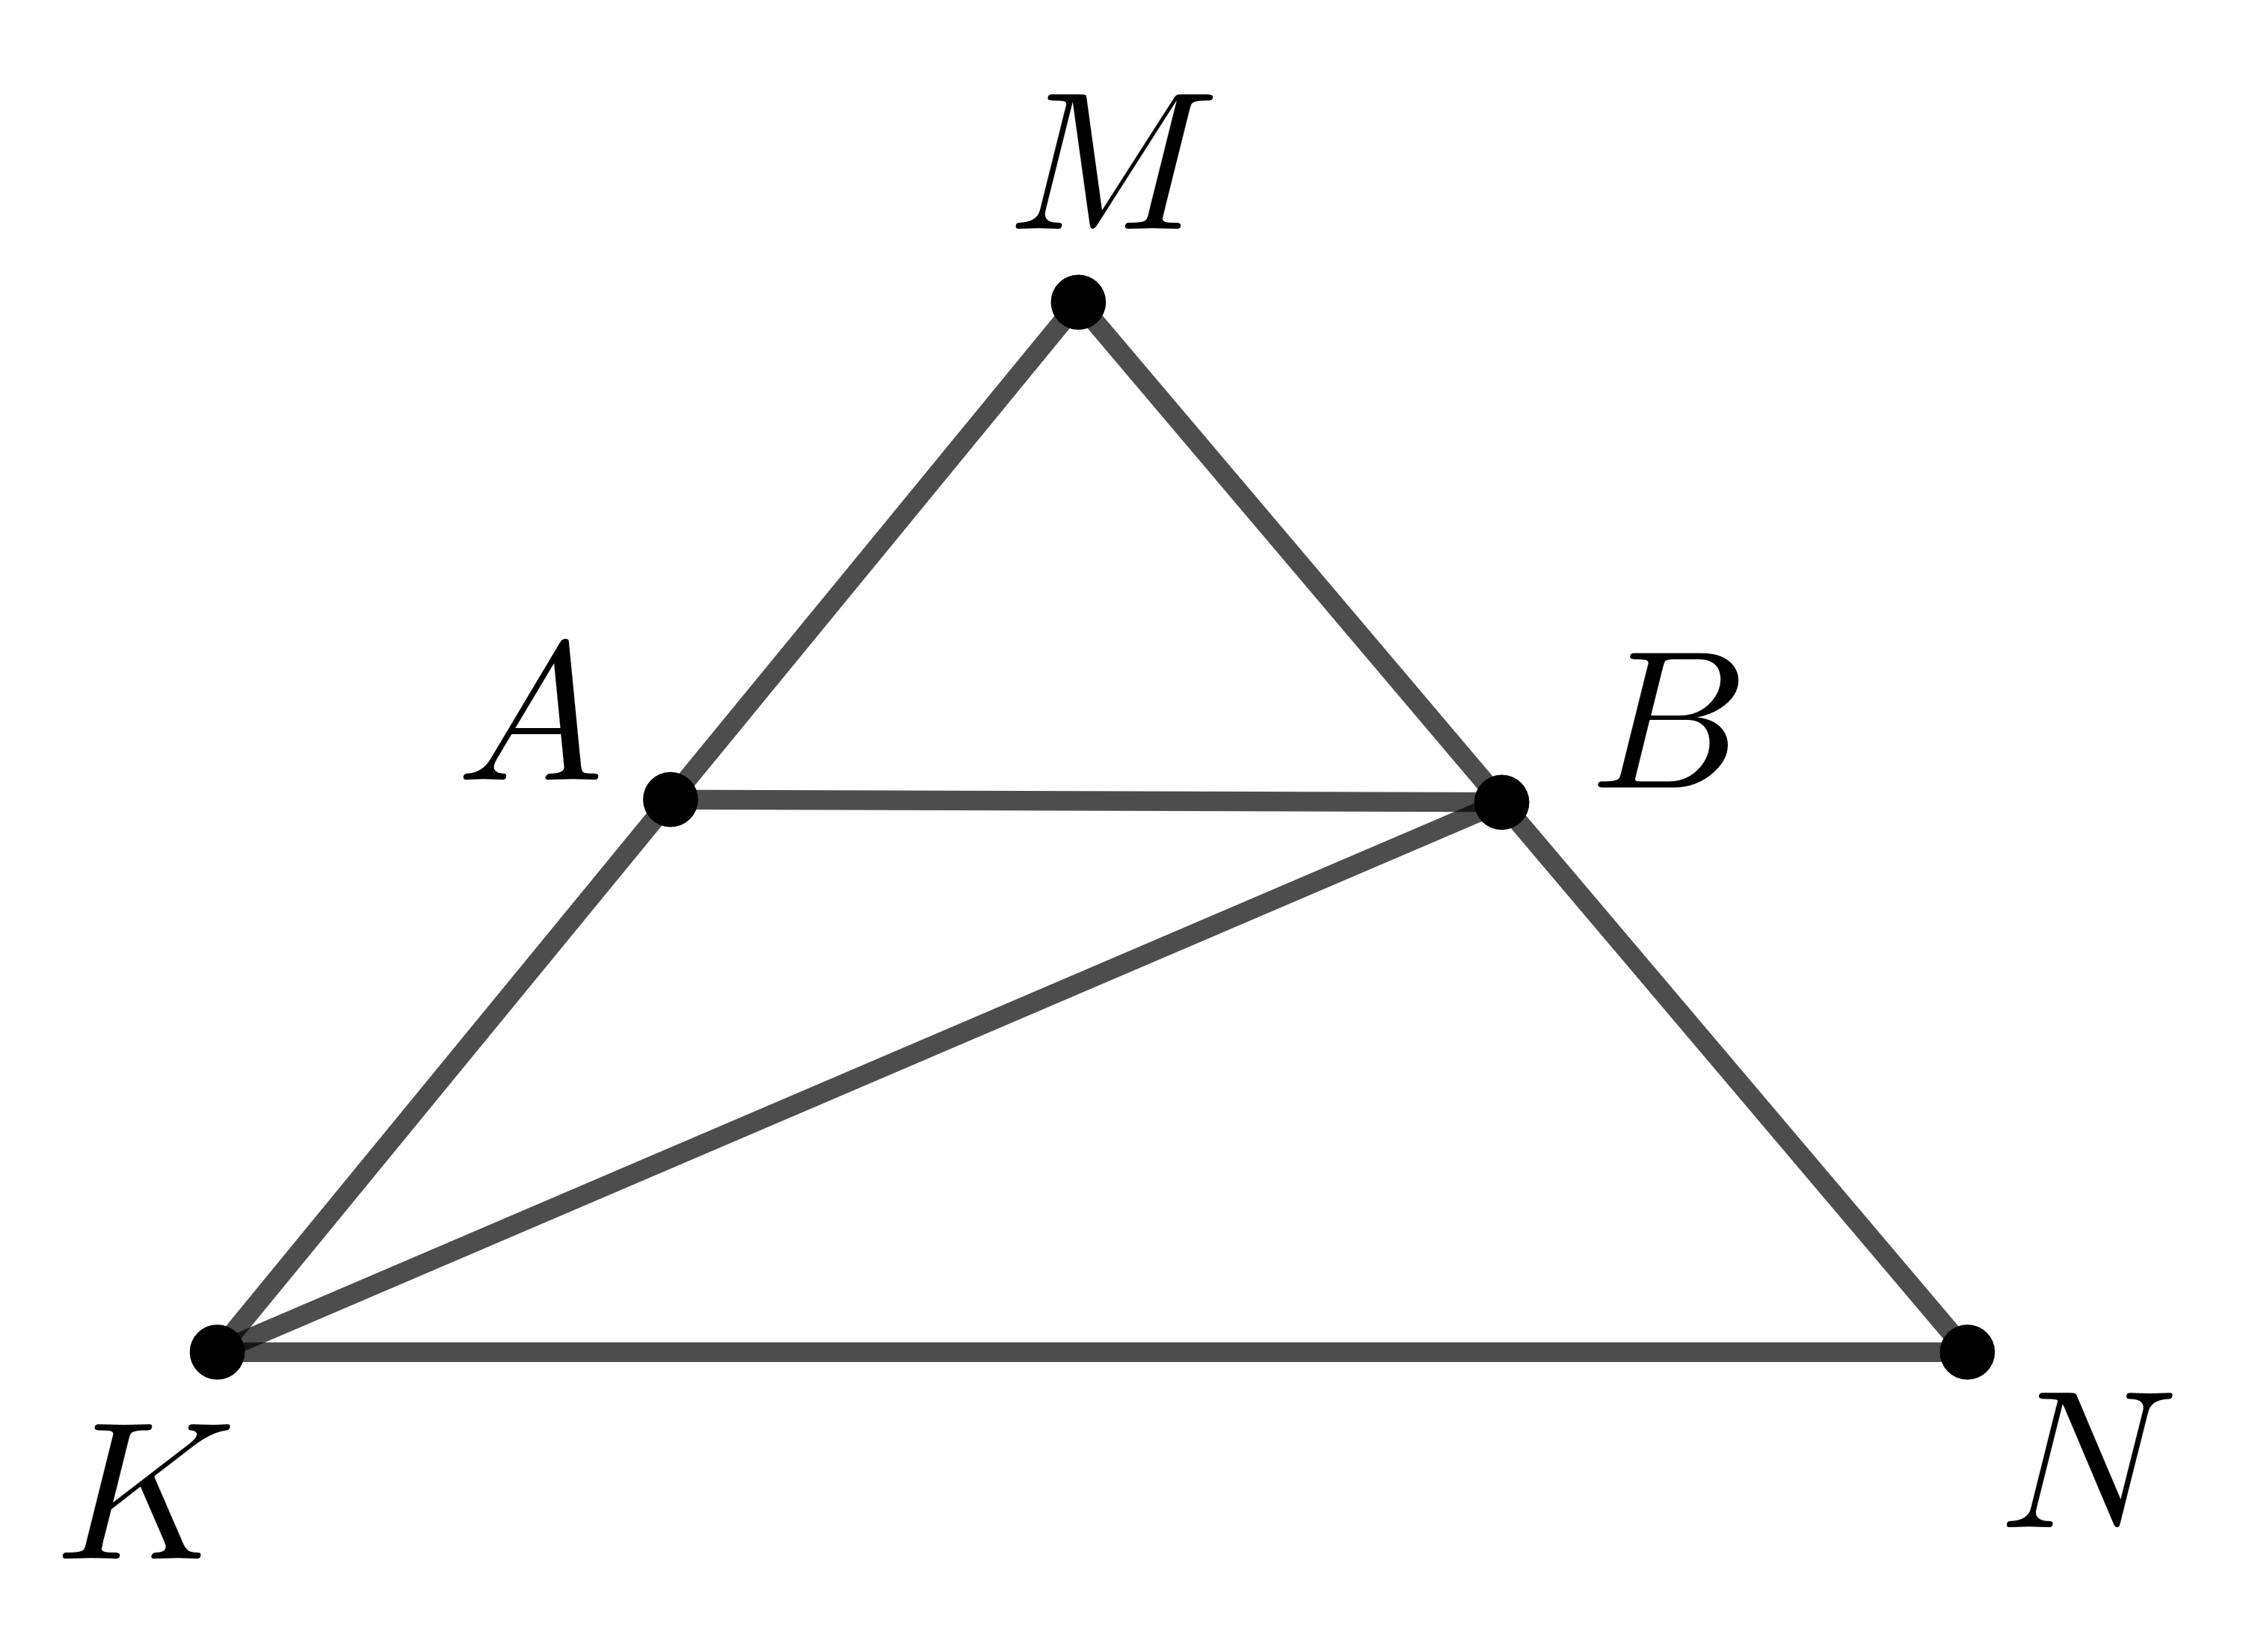
\includegraphics[width=.3\textwidth]{train_exams/20260404/pics/20260404_inzh_7_v1.png}

\smallskip

\samerowans{\begin{problem}{8 (2 балла)}
В треугольнике $ABC$ стороны $AB$ и $AC$ равны. На стороне $AC$ взяли точки $X$ и $Y$ так, что точка $X$ лежит между точками $A$ и $Y$ и $AX = BX = BY$. Найдите $\angle CBY$, если $\angle CAB = 38^\circ$.
\end{problem}}

\smallskip

\begin{problem}{9 (3 балла)}
В треугольнике $ABC$ $\angle C = 90^\circ$, $CD$ — высота треугольника, $BC = 2BD$. Докажите, что $AD = 3DB$.
\end{problem}

\noindent\grid{34}{18}

\smallskip

\begin{problem}{10 (4 балла)}
На рисунке $\angle{ACD}=\angle{BCE}=90^{\text{o}}$. Сравните периметры треугольников ABD и BDE. 
\end{problem}
\smallskip

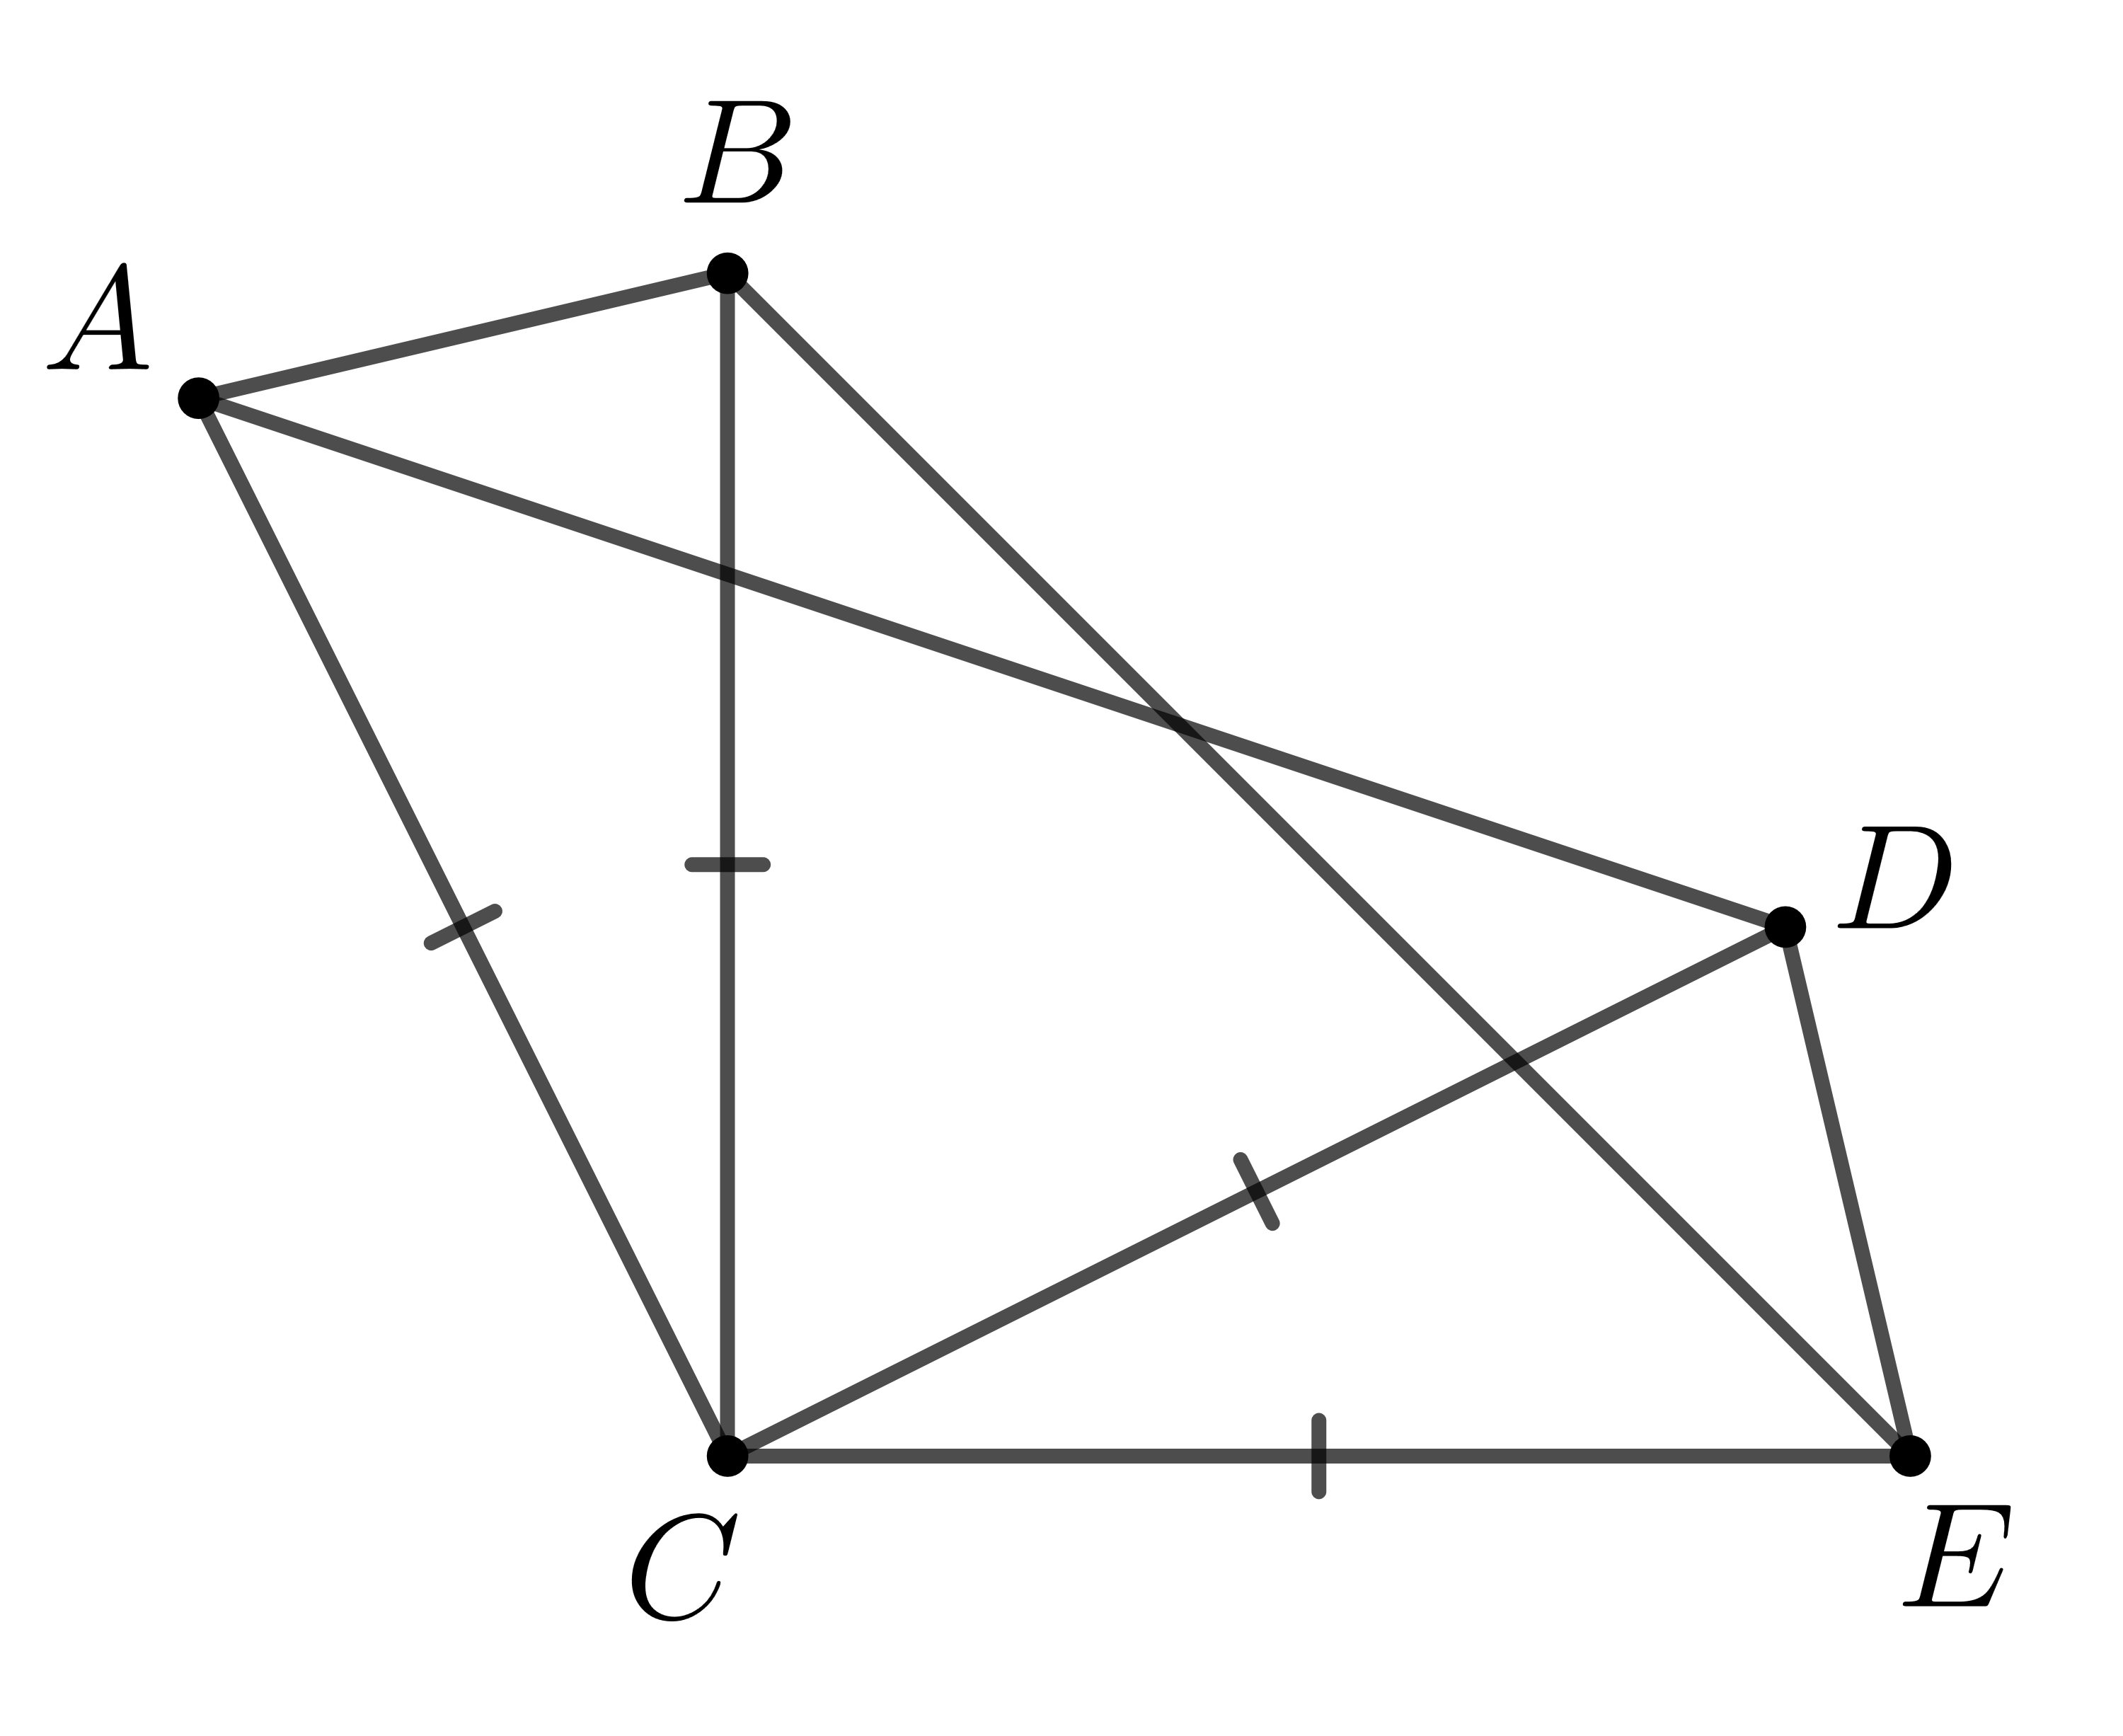
\includegraphics[width=.3\textwidth]{train_exams/20260404/pics/20260404_inzh_10_v1.png}

\smallskip
\noindent\grid{34}{18}
\smallskip

\begin{center}
\textbf{Дополнительная задача}
\end{center}

\begin{problem}{11 (3 балла)}
Решите ОДНО из заданий по выбору. \\
а) Докажите равенство двух треугольников по двум сторонам и высоте, проведённой к одной из этих сторон. \\
б) Найдите значение выражения: $$(x - y)(x + y) - (a - x + y)(a - x - y) - a(2x - a)$$ \\
в) Имеется два сплава меди и свинца. Один сплав содержит 15\% меди, а другой 65\% меди. Сколько нужно взять каждого сплава, чтобы получить 200 г сплава, содержащего 30\% меди?
\end{problem}

\smallskip

\noindent\grid{34}{18}